%
% main.tex -- Paper zum Thema meteor
%
% (c) 2019 Hochschule Rapperswil
%
\chapter{Analyse von Meteor-Echos\label{chapter:meteor}}
\lhead{Analyse von Meteor-Echos}
\begin{refsection}
\chapterauthor{Dominic Hüppi}

Bereits in der Steinzeit, der frühesten Epoche der Menschheitsgeschichte, nahm die Beobachtung von Sonne und Gestirn ihre Anfänge.
Neben der Sonne und dem Mond wirkten Meteore oder umgangssprachlich 'Sternschnuppen' dabei schon immer eine Faszination auf ihre Beobachter aus.
In der Antike galten sie als Vorzeichen für den Tod, im frühen Christentum waren sie ein Zeichen der Seelenerlösung und im Mittelalter überbrachten sie angeblich die Mahnungen Gottes.

Heutzutage, in Zeiten der modernen Astronomie, schauen wir den herabstürzenden Leuchterscheinungen etwas entspannter und objektiver (ausgenommen sind die Flacherdler) entgegen.
Wenn wir heute eine `Sternschnuppe' beobachten gehen Einem die Wünsche in Erfüllung, aber bloss Keinem seinen Wunsch verraten.
Für Astronomen gelten Meteore als wichtige Zeugen aus der Frühzeit des Sonnensystems und für den heute ungemein wichtigen `Influencer' bilden sie ideale Sujets für den nächsten Auftritt in den sozialen Medien.
Und wer hat schon nicht fasziniert dem Himmelgestirn entgegengeblickt und den aufleuchtenden Lichtstrahl romantisiert.

Meteore zeigen sich als überaus interessantes Ereignis.
Das folgende Kapitel bringt weitere Einblicke in die Welt der Meteore und welche Rolle `Wavelets' darin einnehmen.
\begin{figure}
	\centering
	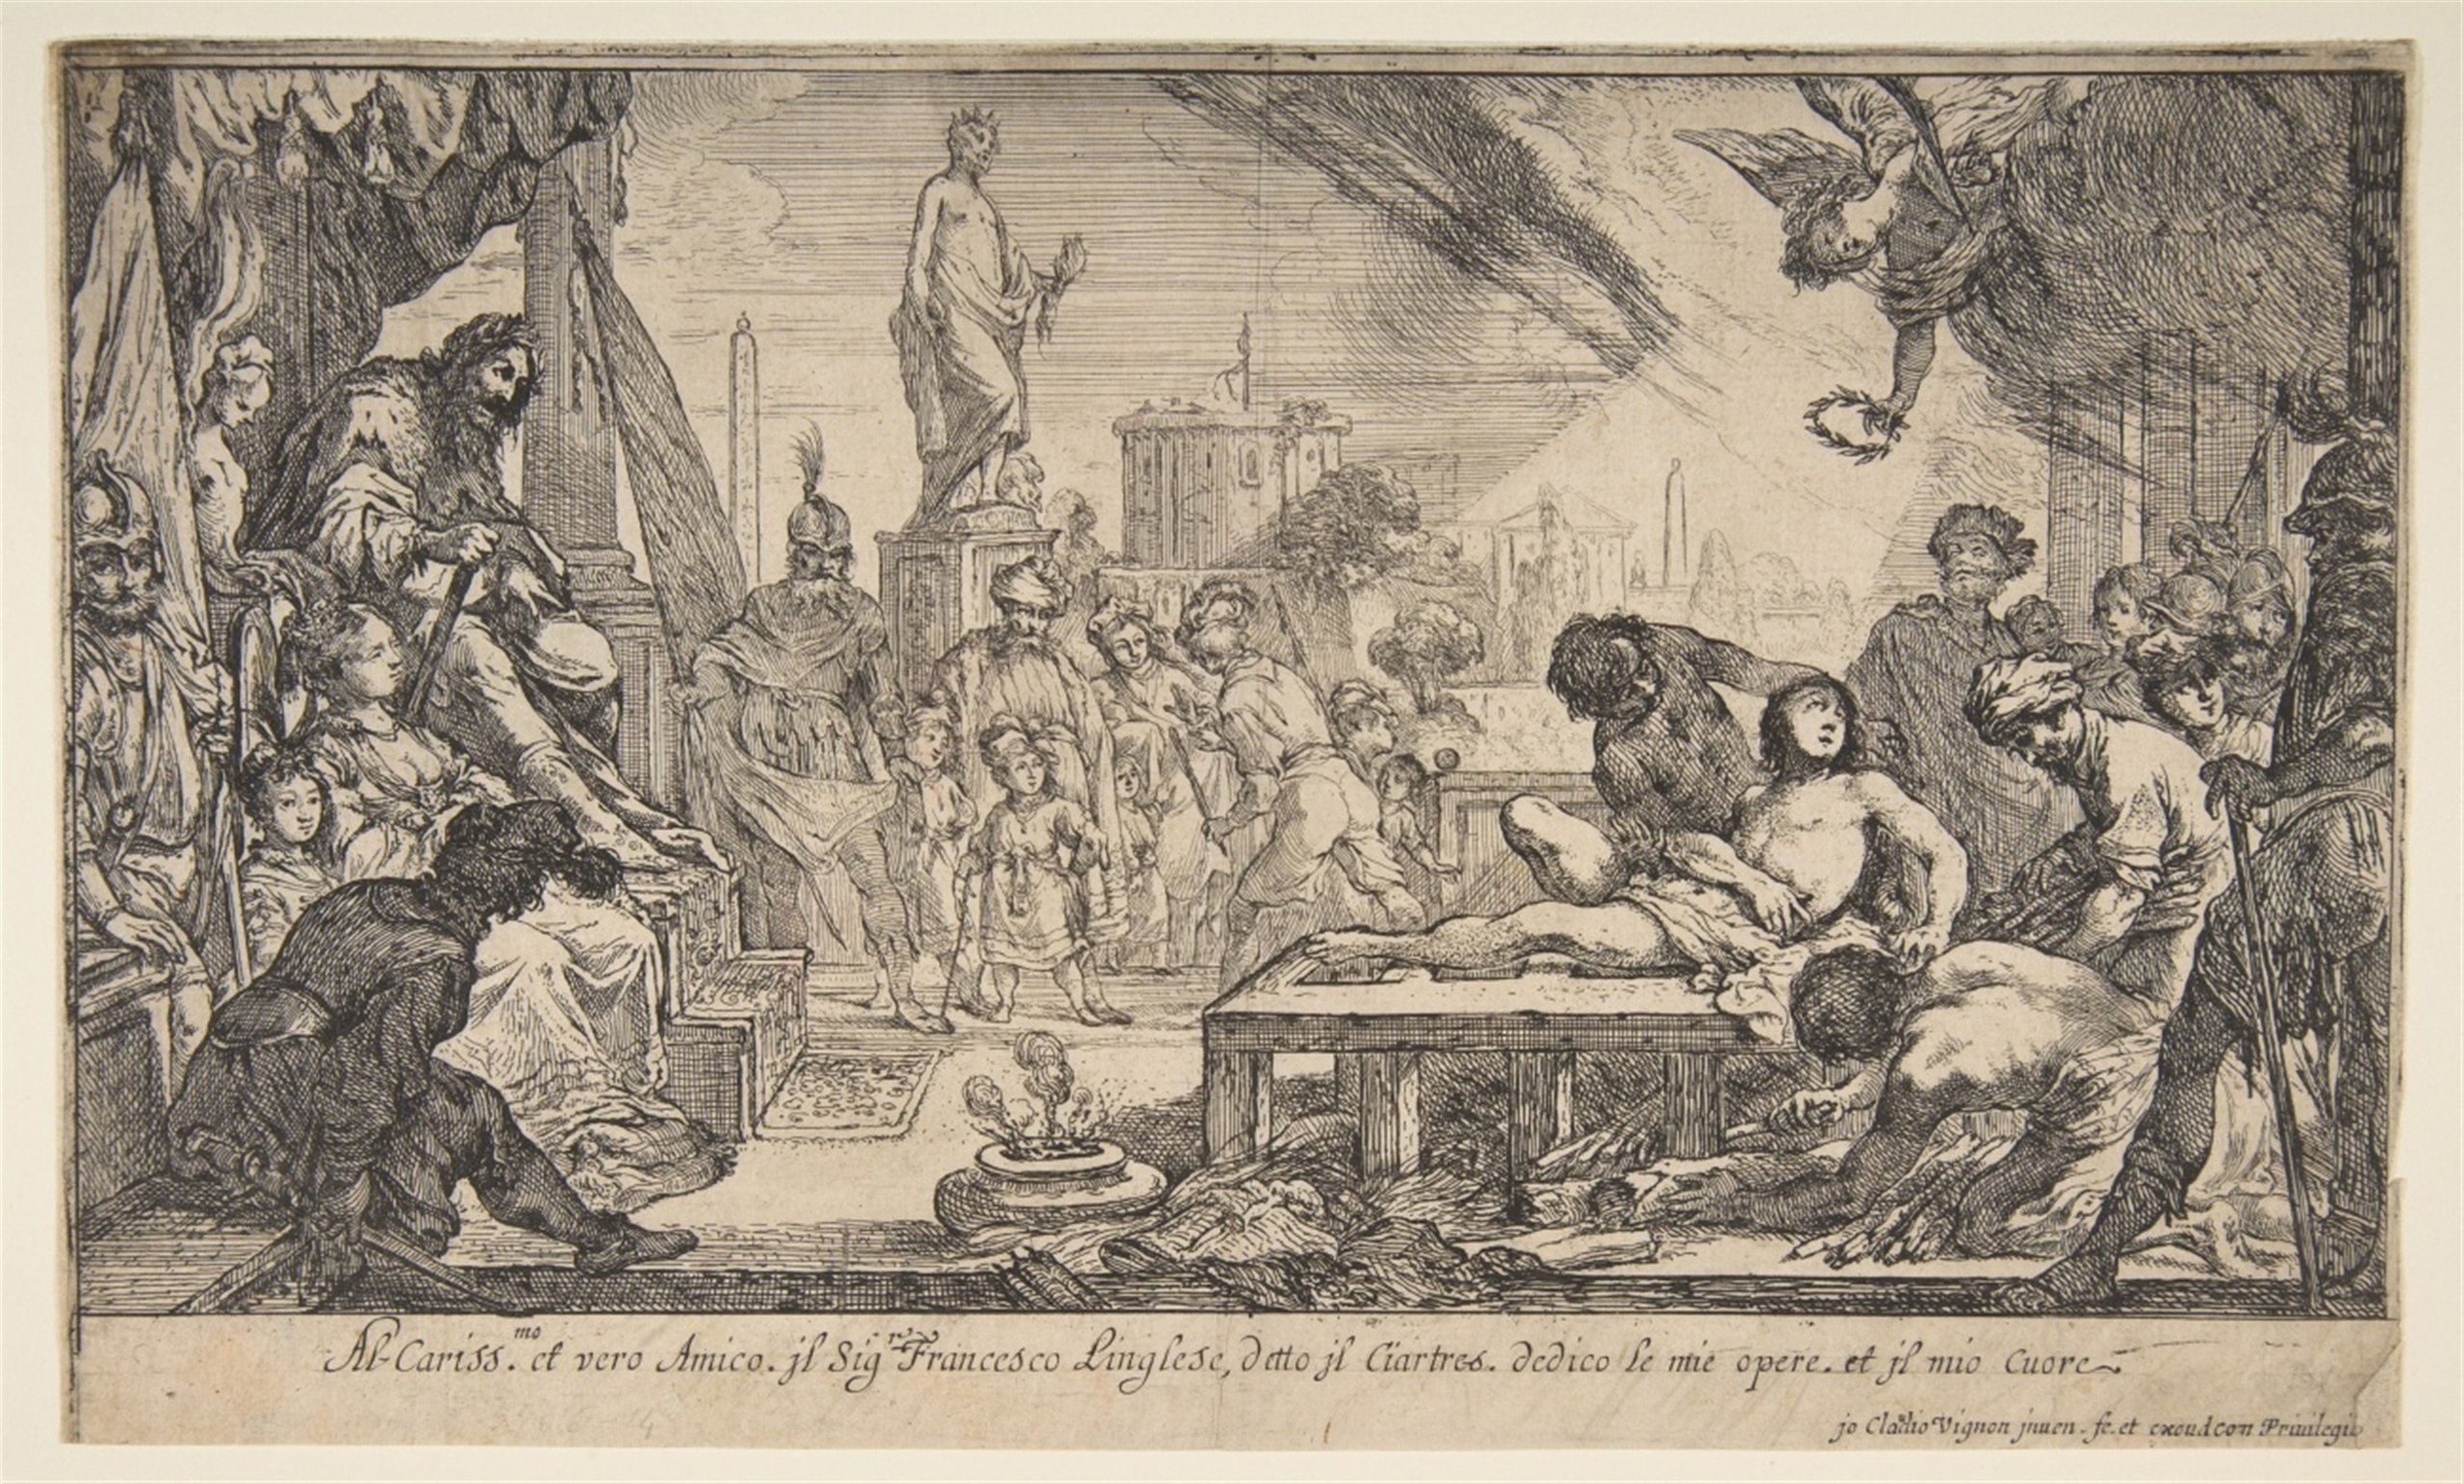
\includegraphics[width=0.9\linewidth]{papers/meteor/images/claudeVignonMartyriumDesHeiligenLaurentius}
	\caption{Martyrium des heiligen Laurentius von Rom im Jahr 258. 
		Hinrichtung auf glühendem Eisenrost, da er sich weigerte den Kirchenschatz dem Kaiser auszuhändigen\cite{buch:joeckle}.
		In der darauffolgenden Nacht trat ein starker Sternschnuppenregen auf, bekannt als Laurentiustränen oder Perseiden. 
		Dieser Meteorstrom ist alljährlich wiederkehrend und kann in der ersten Augusthälfte beobachtet werden\cite{gemaelde:vignon}.}
	\label{fig:claudevignonmartyriumdesheiligenlaurentius}
\end{figure}

\section{Meteore}
\rhead{Abschnitt}

Der Begriff Meteor hat sich über die Zeit verändert. 
Bis zum vorherigen Jahrhundert wurden sämtliche vom Himmel fallende Objekte Meteore genannt. 
Auch Regen, Schnee oder Hagel gehörten dazu. 
Diese Bedeutung des Wortes Meteor ist bis heute in der Wetterkunde als Meteorologie erhalten geblieben.
Allgemein bezeichnet man heute nur noch kleine Objekte, welche beim Eindringen in die Erdatmosphäre eine Lichterscheinung hervorrufen, als Meteore.  
Die Erde ist ständig einem Bombardement aus unzähligen kosmischen Kleinkörpern ausgesetzt. 
Die Kleinkörper werden in die leuchtschwachen `Sternschnuppen' und die leuchtstarken `Feuerkugeln' unterteilt.
Diese beiden Gruppen werden unter dem Begriff Meteor zusammengefasst.
Grössere Objekte, welche die Lichterscheinung einer Feuerkugel hervorrufen, jedoch nicht vollständig in der Atmosphäre verglühen und auf die Erdoberfläche treffen, werden als `Meteorite' bezeichnet.

Entgegen der allgemeinen Annahme, Meteore stürzen wegen der Anziehungskraft der Erde auf sie nieder, ist es viel mehr eine Kollision zweier sich unabhängig bewegender Himmelskörper. 
Die Flugbahn des Meteors wird dabei nur sehr geringfügig durch das Gravitationsfeld der Erde beeinflusst.
Aufgrund der Bahnform ist man heute in der Lage die Objekte ihrer kosmischen Herkunft zuordnen zu können. 
Zwei dieser Herkünfte sind besonders interessant und erklären zudem die Tatsache, dass Meteore oft nicht als Einzelerscheinung auftreten. 
Meteore mit Ellipsen kurzer Umlaufzeit entstammen Planeten oder kleineren Objekten unseres Sonnensystems und werden Planetarische Meteore genannt.
Kometarische Meteore hingegen sind die Begleiterscheinungen eines Kometen. 
Kometen sind im Gegensatz zu Meteoren grosse Himmelskörper mit einem Durchmesser von einigen Kilometern.
Auf ihrer Bahn durchs Sonnensystem ziehen sie einen durch Ausgasen erzeugten leuchtenden Schweif hinter sich her.
Dieser Schweif besteht aus vielen kleinen Objekten, welche sich vom Kometen abscheiden und als kometarische Meteore fortbestehen.
Deshalb ist es nicht verwunderlich, dass gewisse Meteorschauer, wie zum Beispiel der erwähnte Perseiden, zyklisch auftreten\cite{lexikon:meyer}.

Meteore treten mit 30 bis 70 km/s in die Erdatmosphäre ein. 
Die im Durchmesser nur wenige Millimeter grossen Objekte werden aufgrund der grösser werdenden Dichte der Luftschichten Reibung ausgesetzt.
Die auftretenden Kräfte erhitzen den Meteor so stark, dass dieser in circa 80 km Höhe abdampfendes Material hinterlässt.
Dies erzeugt hinter dem herabstürzenden Objekt eine Plasmaspur, welche zusammen mit den Luftatomen eine Rekombination verursacht.
Die Rekombination stellt die Umkehrung der Ionisierung dar. 
Dabei werden elektrisch positiv und elektrisch negativ geladenen Teilchen vereint.
Die bei diesem Prozess entstehende Energie wird durch die Emission von Photonen abgegeben, was zu einer Leuchterscheinung führt\cite{web:brodbeck}.

\newpage
\section{Detektieren von Meteoren}
\rhead{Abschnitt}

Es ist möglich, Meteore mit optischen Systemen zu erfassen. 
Da diese Ereignisse nur kurze Vorläufer haben, gestaltet sich dies als schwierig.
Ebenso ist die Beobachtung stark von den Wetterbedingungen sowie den Lichtverhältnissen abhängig.
Mittels Radio-Echo wird eine kontinuierliche Meteorbeobachtung erreicht. 

\subsection{Elektromagnetische Welle}
In einem Raum kann eine gewisse elektrische Feldenergie einwohnen.
Je grösser die elektrische Feldstärke in diesem Raum ist, desto grösser ist die darin enthaltene elektrische Feldenergie.
Zu dem elektrischen Energiezustand gesellt sich auch der magnetische Feldzustand.
Wo der magnetische Felder bestehen, enthält der Raum magnetische Feldenergie.
Elektrische sowie magnetische Feldenergie sind in den wenigsten Fällen beständig, denn sie haben einen ausgeprägte Neigung zum Zerfall.
Die darin innewohnende Energie kann aber nicht, nach dem Gesetz der Erhaltung der Energie, verschwinden.
Die elektrische Energie kann sich zum Beispiel, wenn Materie anwesend ist, in diese induzieren und bei der damit verbundenen elektrischen `Reibung' in der Materie sich in Wärme umwandeln.
Ist keine Materie in der Umgebung vorhanden, kann sich elektrische Feldenergie in magnetische Feldenergie umwandeln und umgekehrt. 
Die Energie pendelt somit ständig zwischen dem magnetischen und dem elektrischen Zustand hin und her.
Jeder Zerfallsprozess führt dazu, dass bei der Umwandlung der Energie diese sich zerstreut.
Das jeweils entstehende elektrische Sekundärfeld nimmt dabei mehr Platz im Raum in Anspruch als das magnetische Primärfeld.
Somit breiten sich elektromagnetische Felder von ihrem Ursprung her in alle Richtungen aus.
Die Ausbreitung erfolgt im Vakuum mit Lichtgeschwindigkeit.
Die Wellen können sich nicht schneller ausbreiten, da jeder Zerfall des elektrischen oder magnetischen Feldes eine gewisse Trägheit aufweist\cite{buch:meinke}.

Geschwindigkeit mit der sich die elektromagnetische Welle bewegt:
\[
c
=
\frac{1}{\sqrt{\mu\cdot\epsilon}}
\]
Die Phasengeschwindigkeit c hängt von der Permeabilität $\mu$ und der Permittivität $\epsilon$ des Stoffes ab, in der sich die Welle bewegt.

\subsection{Antenne}
Damit eine elektromagnetische Welle entsteht, braucht sie einen Ursprung.
Eine Antenne platziert diesen Ursprung der Welle im freien Raum.
Dabei werden die in Leitern geführten elektromagnetischen Wellen in durch den Raum bewegende Ungeführte gewandelt.
Die Antenne ist das Kopplungselement zwischen Leitungs- und Freiraumwelle.
Wird die Antenne in ihrem Resonanzbereich angeregt, erzeugt diese elektrische sowie magnetische Felder.
Im Nahbereich der Antenne entsteht ein sogenanntes Blindfeld, die Felder bewegen sich von der Quelle weg und wieder zurück, es wird nichts abgestrahlt.
Je grösser die Distanz eines Feldes zur Quelle ist, desto eher entkoppeln sich diese.
Wenn sich der Feldvektor kehrt, verliert das Feld im Randbereich zur Antenne die Kopplung.
Durch die Umkehrung wird das Feld nun von der Antenne abgestoßen und eine elektromagnetische Welle wird in den Raum abgestrahlt.
Der selbe Prozess funktioniert auch entgegengesetzt und die Antenne somit als Empfänger\cite{buch:unger}.

\subsection{Ausbreitung der Welle}
Die Ausbreitung von elektromagnetischen Wellen in Erdnähe wird durch die Mitwirkung der Erdoberfläche sowie den Eigenschaften der Atmosphäre verkompliziert.
Gerade Kurzwellen erreichen nur geringe Reichweiten.
Die Reichweite von Langwellensendern kann dagegen bis zu 1000 Kilometern betragen.
Der Erdboden wirkt als Verbund aus schlechten elektrischen Leitern und Nichtleitern. 
Je weiter die Welle sich am Erdboden nach fortbewegt, desto mehr Energie gibt sie an diesen ab.
Da ausserdem mit wachsender Frequenz die Zahl der Verschiebungsströme pro Zeit zunimmt, nimmt auch der Energieverlust an den Erdboden zu.
Mit einer Richtantenne kann diesen Erdbodenverlusten vorgebeugt werden, da die Wellen sich gebündelt fortbewegen und möglichst wenig Berührung zum Erdboden haben.

Gegenüber dem Erdboden befindet sich die Atmosphäre.
Unsere Erde ist diversen Strahlungen aus dem Kosmos ausgesetzt.
Diese Strahlungen werden in der Atmosphäre fast vollständig absorbiert.
Die Luftmoleküle nehmen bei dieser Absorption Strahlungsenergie auf.
Ein resultierender Effekt daraus ist, dass sich Elektronen aus den Atomen abspalten und diese freien Elektronen an anderen Atomen ansammeln.
In der hohen Atmosphäre sind daher positive und negative Ionen und freie Elektronen vorhanden.
Dieser Bereich befindet sich in circa 70 bis 300 km Höhe und wird Ionosphäre genannt.
Darüber befinden sich zu wenige Atome, welche ionisiert werden könnten und darunter ist die Intensität der energetischen Strahlung bereits zu stark durch die Atmosphäre geschwächt.
Durch den niedrigen Druck in grossen Höhen wird die freie Beweglichkeit der geladenen Teilchen ermöglicht.
Diese Vorgehen in der Ionosphäre führen dazu, dass elektromagnetische Wellen gewisser Frequenzen an ihr, wie an einer leitenden Wand, reflektiert werden.
Dies kann bei starker Ladungskonzentration zu einer Totalreflexion führen. 
Oberhalb der Frequenz von 30MHz reicht die erforderliche Ladungskonzentration für eine Reflexion nicht mehr aus\cite{buch:meinke}.


\section{Auswertung der Radio-Signale}
\rhead{Abschnitt}

In meiner Arbeit möchte ich Aufzeichnungen von Radaranlagen auswerten und überprüfen wie gut sich die Wavelet Transformation dafür eignet.
Die Herausforderung ist es geeignete Radardaten zu erhalten, aufzubereiten und eine geeignete Wavlet Transformation durchzuführen.
Aus dem daraus Resultierenden Bild möchte ich folgende Informationen gewinnen können:
\begin{itemize}
	\item Wann ist ein Meteor in die Atmosphäre eingetreten
	\item Welche zusätzlichen Aussagen können über einen detektierten Meteor getroffen werden 
	\item Welche anderen Objekte können erkannt und zugeordnet werden können
	\item Falls andere Flugobjekte (zB. Flugzeuge) erkannt werden, können Aussagen zu deren Geschwindigkeit gemacht werden
\end{itemize}

\subsection{Radardaten}
Für die Versuche werden auf die Daten des BRAMS (Belgian RAdio Meteor Stations) Projektes zugegriffen.
Das Netzwerk besteht aus einem Sender und circa 30 Empfängern.
Verschiedene Institutionen und auch Private studieren damit den Meteor-Niedergang über Belgien.
Durch das Erstellen eines Benutzerkontos kann jeder frei über die gesammelten Daten verfügen.
Die Empfangsdaten einer Station können als Audiofile im .wav Format bezogen werden und dauern fünf Minuten.

\newpage
\subsection{Signalanalyse}
Mit dem Computerprogramm `Matlab' wird die Signalverarbeitung und Analyse vorgenommen.
Folgend werden wichtige Ausschnitte aus dem Matlab-Sourcecode gezeigt und erklärt.
Das Signal stammt von einer Messung des BRAMS Netzwerk und besitzt eine Dauer von circa 2 Minuten.
Es kann ein beliebiger Satz Daten des Netzwerks verarbeitet werden.

Die Audiofiles im .wav Format können wie folgt eingelesen werden:
\begin{lstlisting}
dataname    = 'PFAD_ZU_FILE';
[sig,Fs]    = audioread(dataname);
info        = audioinfo(dataname);
\end{lstlisting}
Die Abtastrate `Fs' beträgt 5512,5 Punkte pro Sekunde.
Aus der Variable `info' können Informationen wie zB. die Dauer entnommen werden. 

Der interessante Bereich liegt zwischen 1050 und 1150 Herz.
Daher wird ein Bandpassfilter für diesen Bereich eingesetzt:
\begin{lstlisting}
frrange     = [1050 1150];
sig         = bandpass(sig, frrange, Fs);
\end{lstlisting}

Signalanteile mit Amplitude unter 0.025 nach Matlab normalisierter Wert werden auf 0 gesetzt.
\begin{lstlisting}
sig(sig<0.025) = 0;
\end{lstlisting}

Um eine Referenz zu haben, sowie einen Vergleich machen zu können, wird das Signal zuerst mit einer gefensterten Fourier-Transformation dargestellt. 
\begin{lstlisting}
figure('Name','GFFT');
SNR = 100;
wind = 2^14;
nlap = 14776;
nfft = 2^14;
[s, f, tsp, psd] = spectrogram(sig,wind,nlap,nfft,Fs,'MinThreshold',-SNR,'yaxis');
imagesc(ts,f,10*log10(psd));
axis xy; 
axis tight; 
view(0,90);
xlabel('Time (secs)');
ylabel('Frequency(HZ)');
ax = gca;
ax.YLim = frrange;
\end{lstlisting}

\newpage
Die gesetzten Werte um die Transformation auszuführen wurden durch Versuche entdeckt. 
Die Beschreibung der Funktion `spectrogram' ist in den Dokumentation von Matlab enthalten.
Mit der Funktion `imagesc' wird das Ergebnis grafisch dargestellt.
Dargestellt wird die spektrale Leistungsdichte.

\begin{figure}[h]
	\centering
	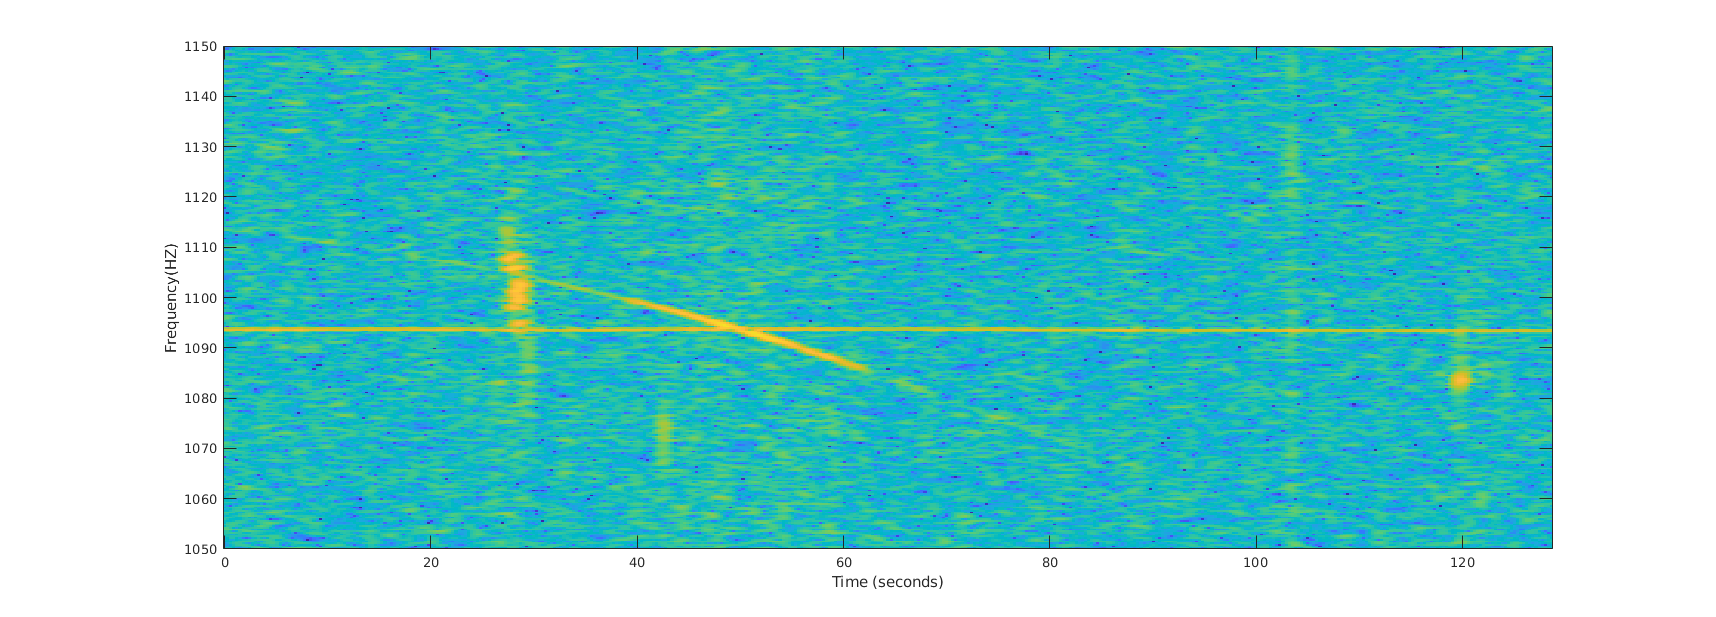
\includegraphics[width=\linewidth]{papers/meteor/images/signal_gfft.png}
	\caption{Die gefensterte Fourier-Transformation mit Matlab grafisch dargestellt}
	\label{fig:signalmitgfft}
\end{figure}
In der Grafik lassen sich drei verschiedene charakteristische Signaturen unterscheiden:
\begin{itemize}
	\item Kurze starke Hervorhebungen über ein breites Frequenzband.
	\item S-Kurven-ähnliche  Hervorhebungen.
	\item Eine leichte Hervorhebung bei nur einer Frequenz über die gesamte Zeit.
\end{itemize}
 
Mit der kontinuierlichen Wavelet-Transformation CWT wird nun versucht ein vergleichbares Bild des Radarsignals zu erzeugen.
Das `Gabor Wavelet' oder auch `Morlet' genannt hat bei den Versuchen gute Ergebnisse erzielt.
\begin{lstlisting}
wav = 'amor';
cfs = cwt(sig,wav,Fs);
\end{lstlisting}
Der Matlab Funktion `cwt' werden als Parameter das Radarsignal sig, Das Gabor Wavelet amor und die Abtastrate übergeben.
Als Rückgabe erhalten wir eine Koeffizienten-Matrix.

Diese Koeffizienten-Matrix muss noch modifiziert werden.
\begin{lstlisting}
tmp1 = abs(cfs);
t1 = size(tmp1,2);
tmp1 = tmp1';
maxv = max(tmp1);
maxvArray = maxv(ones(1,t1),:);
tmp1 = 240*(tmp1./maxvArray);
tmp2 = 1+fix(tmp1);
tmp2 = tmp2';
\end{lstlisting}
Die Werte der Matrix sind komplex.
Mit der Funktion `abs' erhalten wir den Betrag.

\newpage
Die Koeffizienten-Matrix stellen wir mit der Funktion `wscalogram' über die Zeit dar.
\begin{lstlisting}
wscalogram('image',tmp2,'xdata',ts);
title('Continuous Transform, absolute coefficients');
set(gca,'YDir','reverse')
ax = gca;
ax.YLim = [60 140];
colormap jet;
\end{lstlisting}
Das Resultat ist eine Grafik welche zu jedem Zeitpunkt zeigt wie gut das Gabor Wavelet in welcher Streckung mit dem Signal korreliert. 

\begin{figure}[h!]
	\centering
	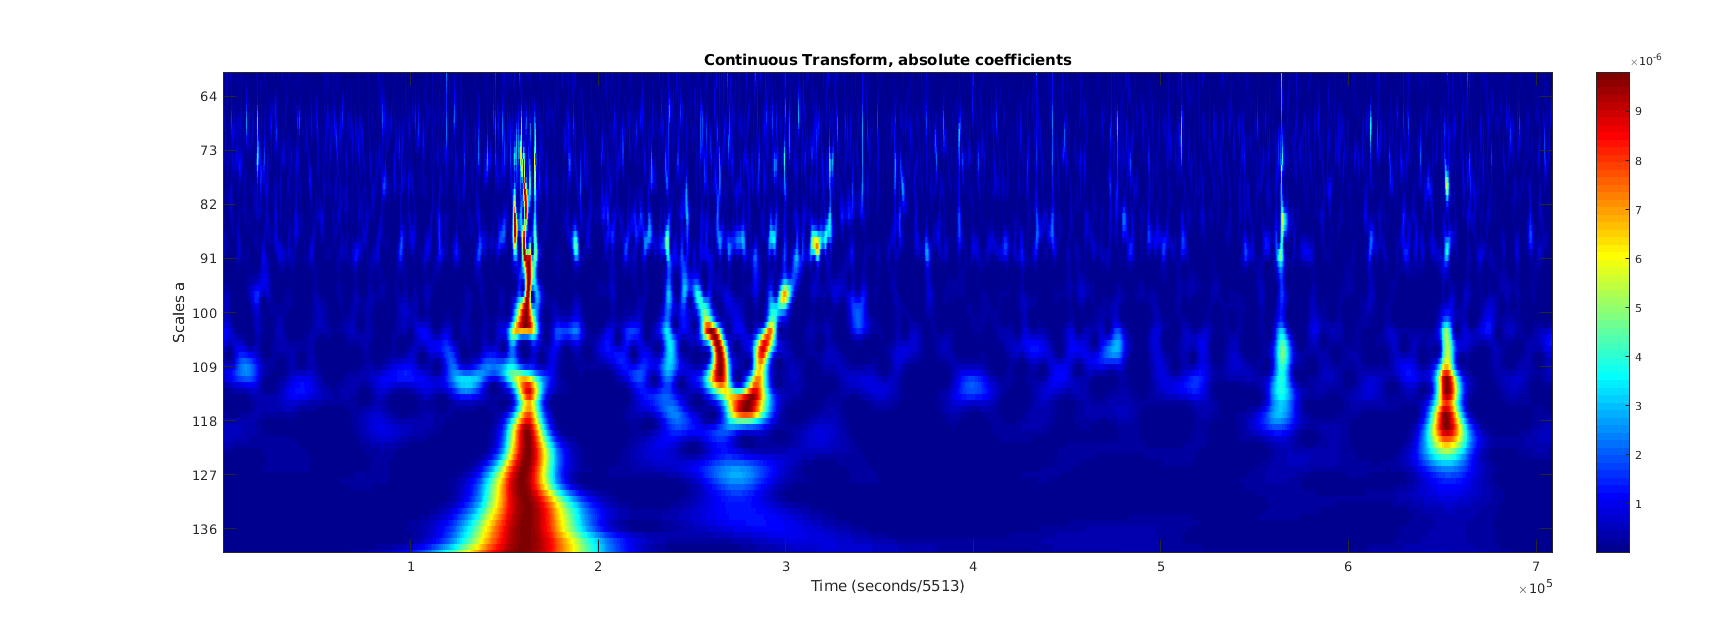
\includegraphics[width=\linewidth]{papers/meteor/images/signal_wscalo.png}
	\caption{Die kontinuierliche Wavelet-Transformation mit Matlab grafisch dargestellt}
	\label{fig:signalmitwscalo}
\end{figure}
In der Grafik lassen sich zwei verschiedene charakteristische Signaturen unterscheiden:
\begin{itemize}
	\item Kurze starke Hervorhebungen über einen breiten Bereich an verschiedenen Streckungen.
	\item V-Kurven-ähnliche  Hervorhebungen.
\end{itemize}

\newpage
\subsection{Auswertung}
Signaturen der 1.Art sind mit beiden Methoden erkennbar.
Da diese nur wenige Sekunden dauern und ein breites Frequenzband reflektieren deuten sie auf Meteore hin.
Man kann annehmen, dass je grösser der Partikelstrom des Meteors ist, desto stärker zeigt sich seine Signatur nach der Wavelet-Transformation.
Allerdings trifft diese Aussage nur zu, wenn wir annehmen, dass alle aufgezeichneten Meteore gleich weit entfernt sind.

Signaturen der 2.Art sind mit beiden Methoden erkennbar.
Jedoch zeigt sich hier ein erstaunlicher Unterschied.
Nach der gefensterten Fouriertransformation sind die Signaturen S-Förmig.
Diese S-Förmigen Signale deuten auf sich `langsamer' bewegende Flugobjekte, wie in den meisten Fällen Flugzeuge hin.
Die charakteristische Form entsteht auf Grund des optischen Dopplereffektes. 
Bewegt sich ein Objekt auf die Empfangsstation zu, werden die reflektierenden Radarwellen gestaucht, die empfangene Frequenz erscheint höher.
Bewegt sich ein Objekt von der Empfangsstation weg, werden die reflektierenden Radarwellen in die Länge gezogen und die empfangene Frequenz erscheint tiefer.

Resultierende Frequenz aufgrund des optischen Dopplereffektes beim Annähern von Sender und Empfänger:
\[
f_E
=
f_S\cdot\sqrt{\frac{1+\frac{v}{c}}{1-\frac{v}{c}}}
\]

Resultierende Frequenz aufgrund des optischen Dopplereffektes beim Entfernen von Sender und Empfänger:
\[
f_E
=
f_S\cdot\sqrt{\frac{1-\frac{v}{c}}{1+\frac{v}{c}}}
\]
\(f_E\) ist die empfangene Frequenz.
\(f_S\) ist die abgestrahlte Frequenz.
v ist die relative Geschwindigkeit des Senders zum Empfänger.
c ist die Phasengeschwindigkeit der elektromagnetischen Welle.

Nach der Wavelet-Transformation zeigt sich uns ein leicht anderes Bild.
Die S-förmigen Signale gleichen eher einem V.
Die Frequenz des Signales nimmt ab und anschliessend wieder zu.
Gleiche Ergebnisse tauchen mit unterschiedlichen Wavelets und Signalen ebenfalls auf.

Signaturen der 3.Art sind nur mit der Fourier-Methode zu erkennen.
Es handelt sich dabei um das Sendesignal, welches ungehindert zur Ionosphäre gelangt, an ihr reflektiert wird und ungehindert beim Empfänger eintrifft.
Diese Signatur ist nach der Wavelet-Transformation nicht mehr zu erkennen.
Es scheint, als würde eben jenes Signal schlecht mit unseren eingesetzten Wavelets korrelieren. 

\newpage
\subsection{Erklärung der Anomalien}
Die Ergebnisse mit der Wavelet-Transformation sind höchst erstaunlich und stimmen nicht mit den Ergebnissen der gefensterten Fourier-Transformation und meinen Erwartungen überein.
Es stellt sich die Frage, warum das Trägersignal, dass eine Frequenz von circa 1093 Hz hat, nicht nach der Wavelet-Transformation noch zu erkennen ist.
Des weiteren muss die Frequenz, eines sich vom Empfänger entfernenden Objektes, nach Doppler abnehmen.
Nach der Wavelet-Transformation sieht es jedoch so aus, als würde die Frequenz des zu analysierenden Signales erst ab- und anschliessend wieder zunehmen.

Um diesen Phänomenen auf den Grund zu gehen, wurden mit verschiedenen künstlich erzeugten Signalen Analysen durchgeführt.
Um das Verhalten des Trägersignals nachzuvollziehen, werden Signale mit gleichbleibender Frequenzen von 100 Hz bis 2400 Hz untersucht:
\begin{figure}[h]
	\centering
	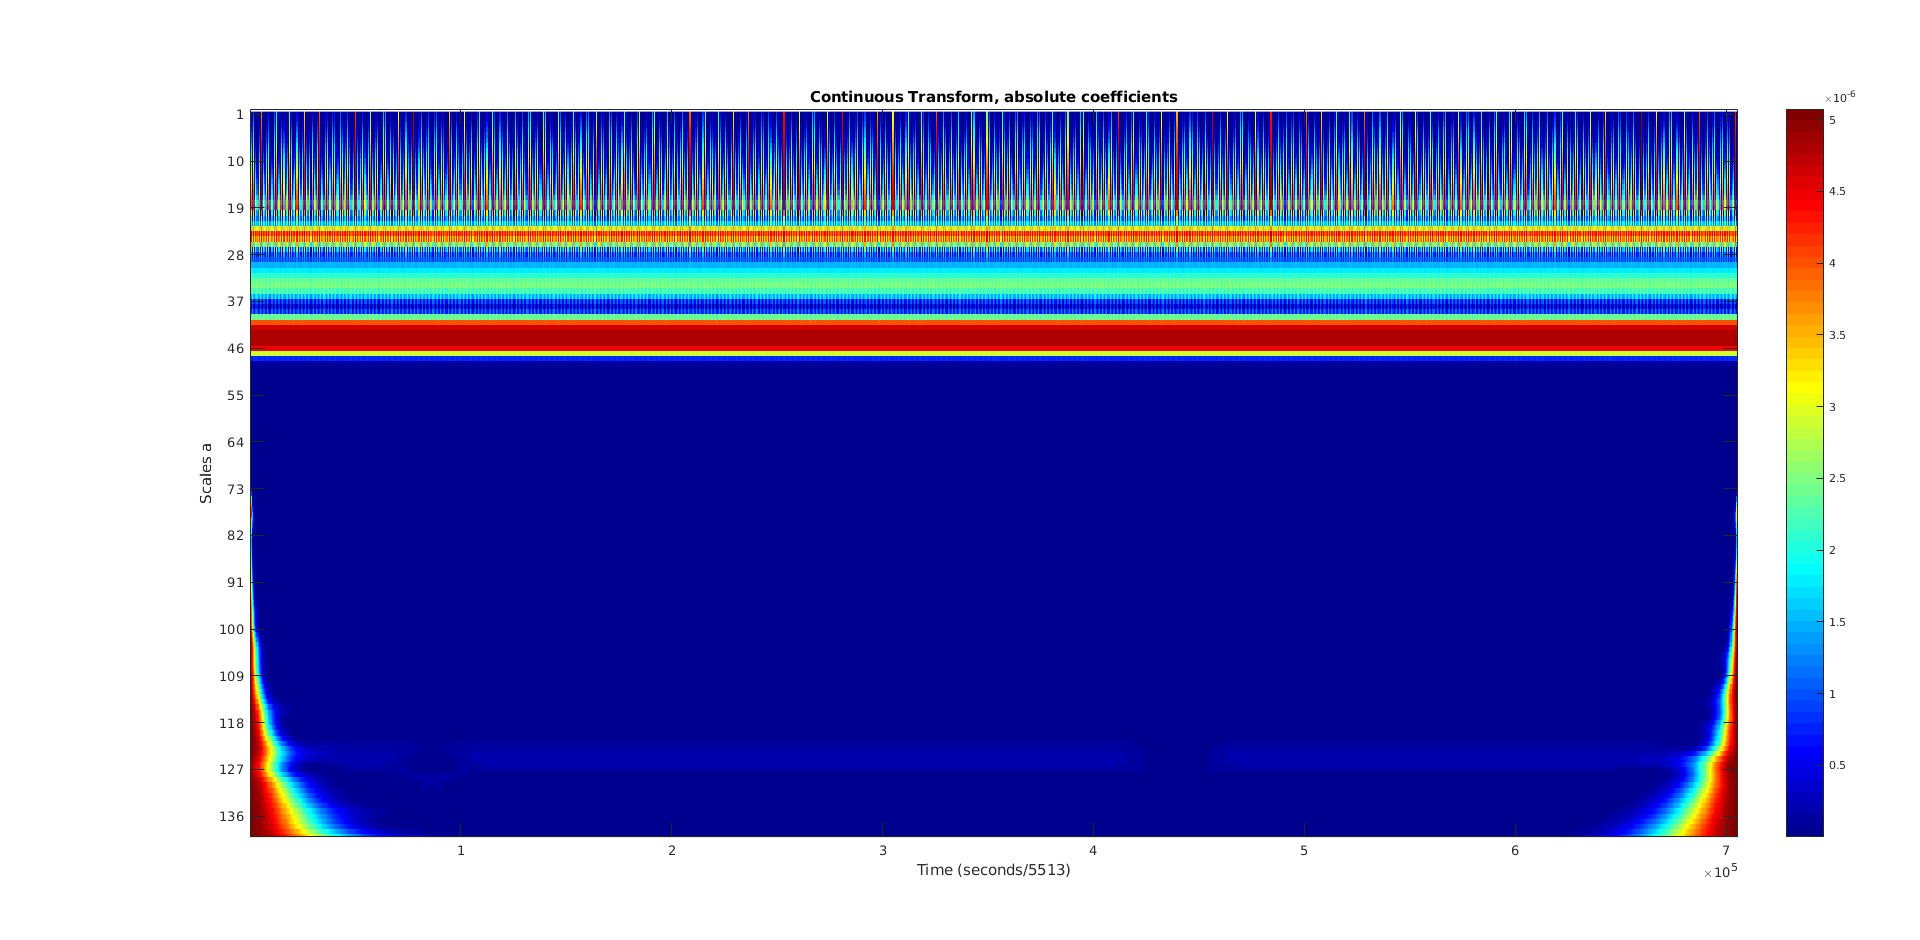
\includegraphics[width=0.9\linewidth]{papers/meteor/images/anomalie/beam/cwt_0100hz.png}
	\caption{100 Herz Sinussignal mit kontinuierliche Wavelet-Transformation}
	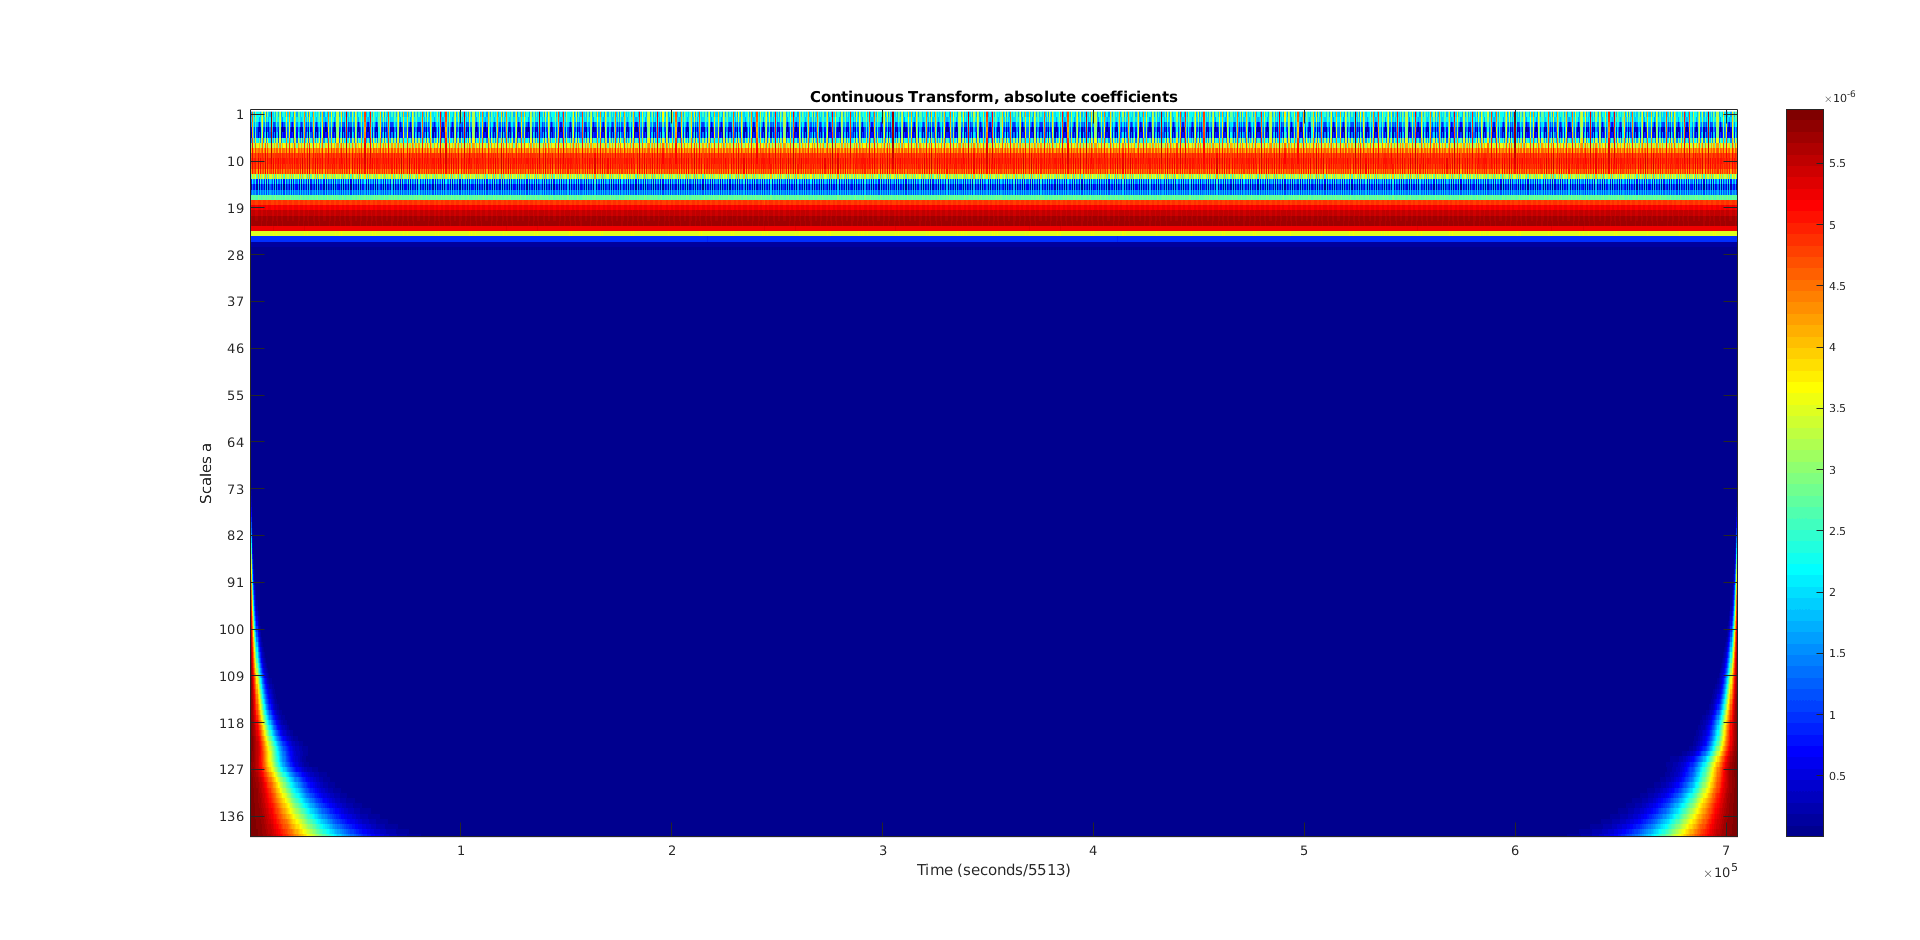
\includegraphics[width=0.9\linewidth]{papers/meteor/images/anomalie/beam/cwt_0500hz.png}
	\caption{500 Herz Sinussignal mit kontinuierliche Wavelet-Transformation}
	\label{fig:cwt_anomalie_beam_1}
\end{figure}
\newpage
\begin{figure}[h]
	\centering
	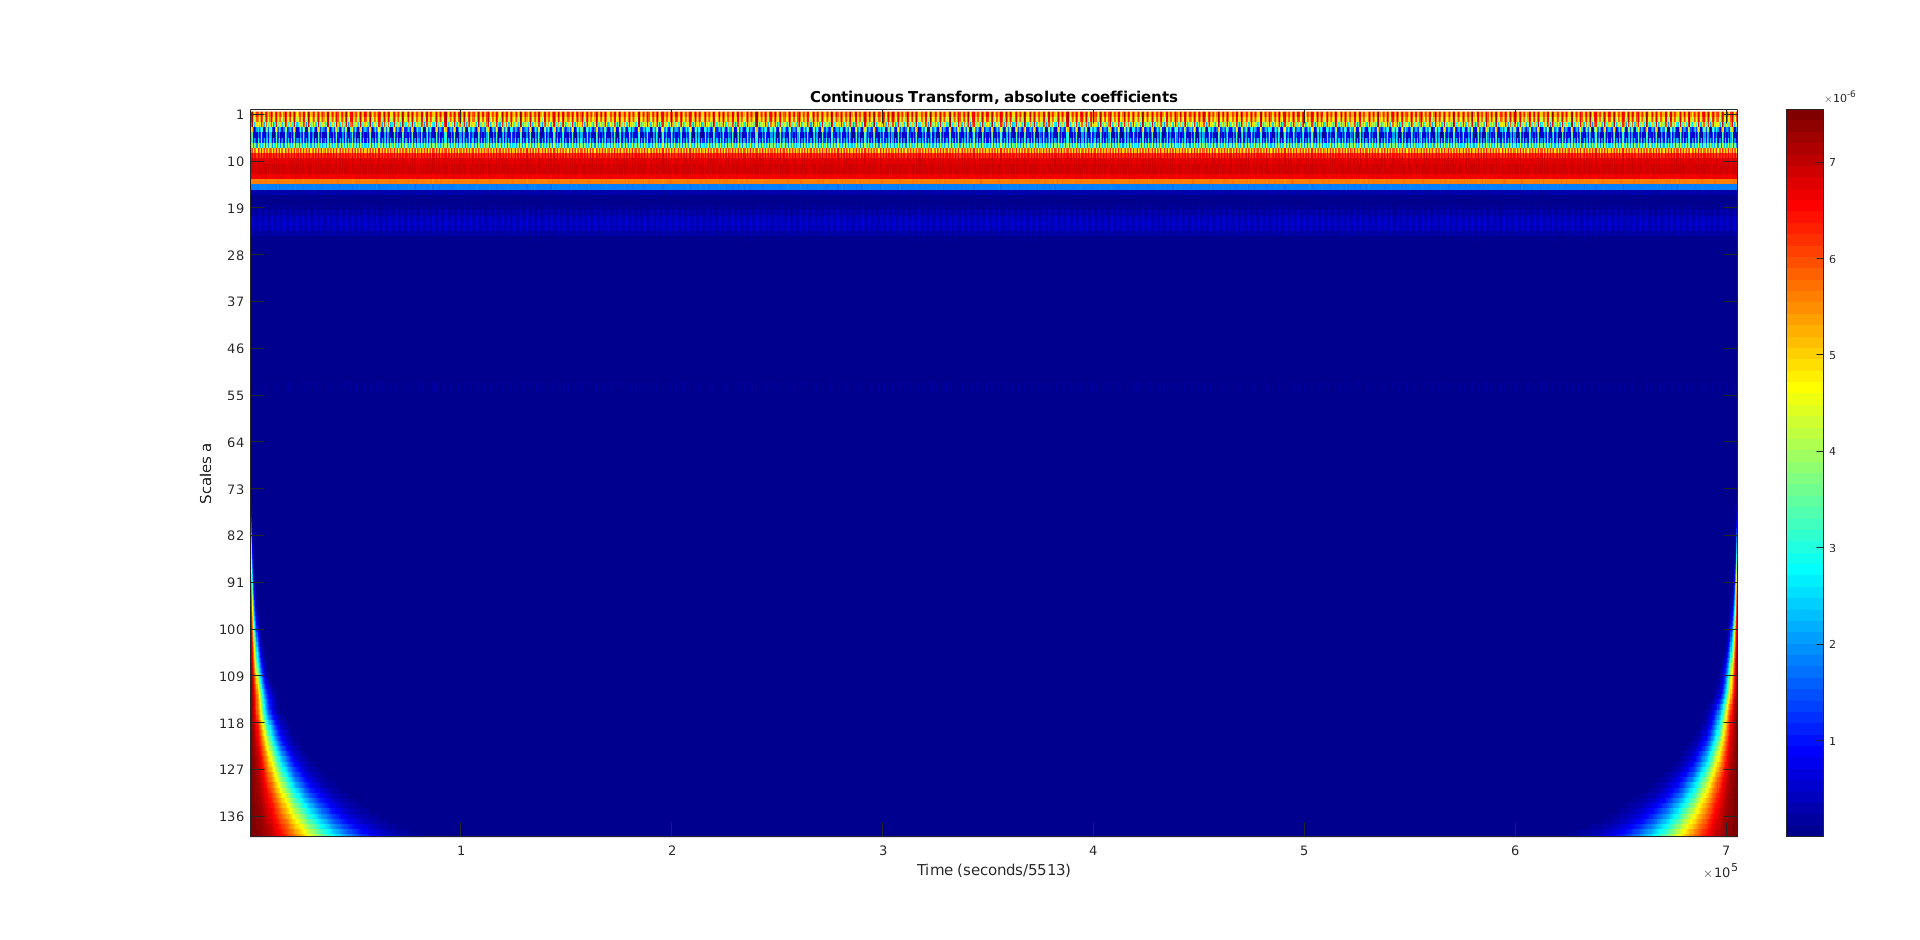
\includegraphics[width=0.9\linewidth]{papers/meteor/images/anomalie/beam/cwt_1000hz.png}
	\caption{1000 Herz Sinussignal mit kontinuierliche Wavelet-Transformation}
	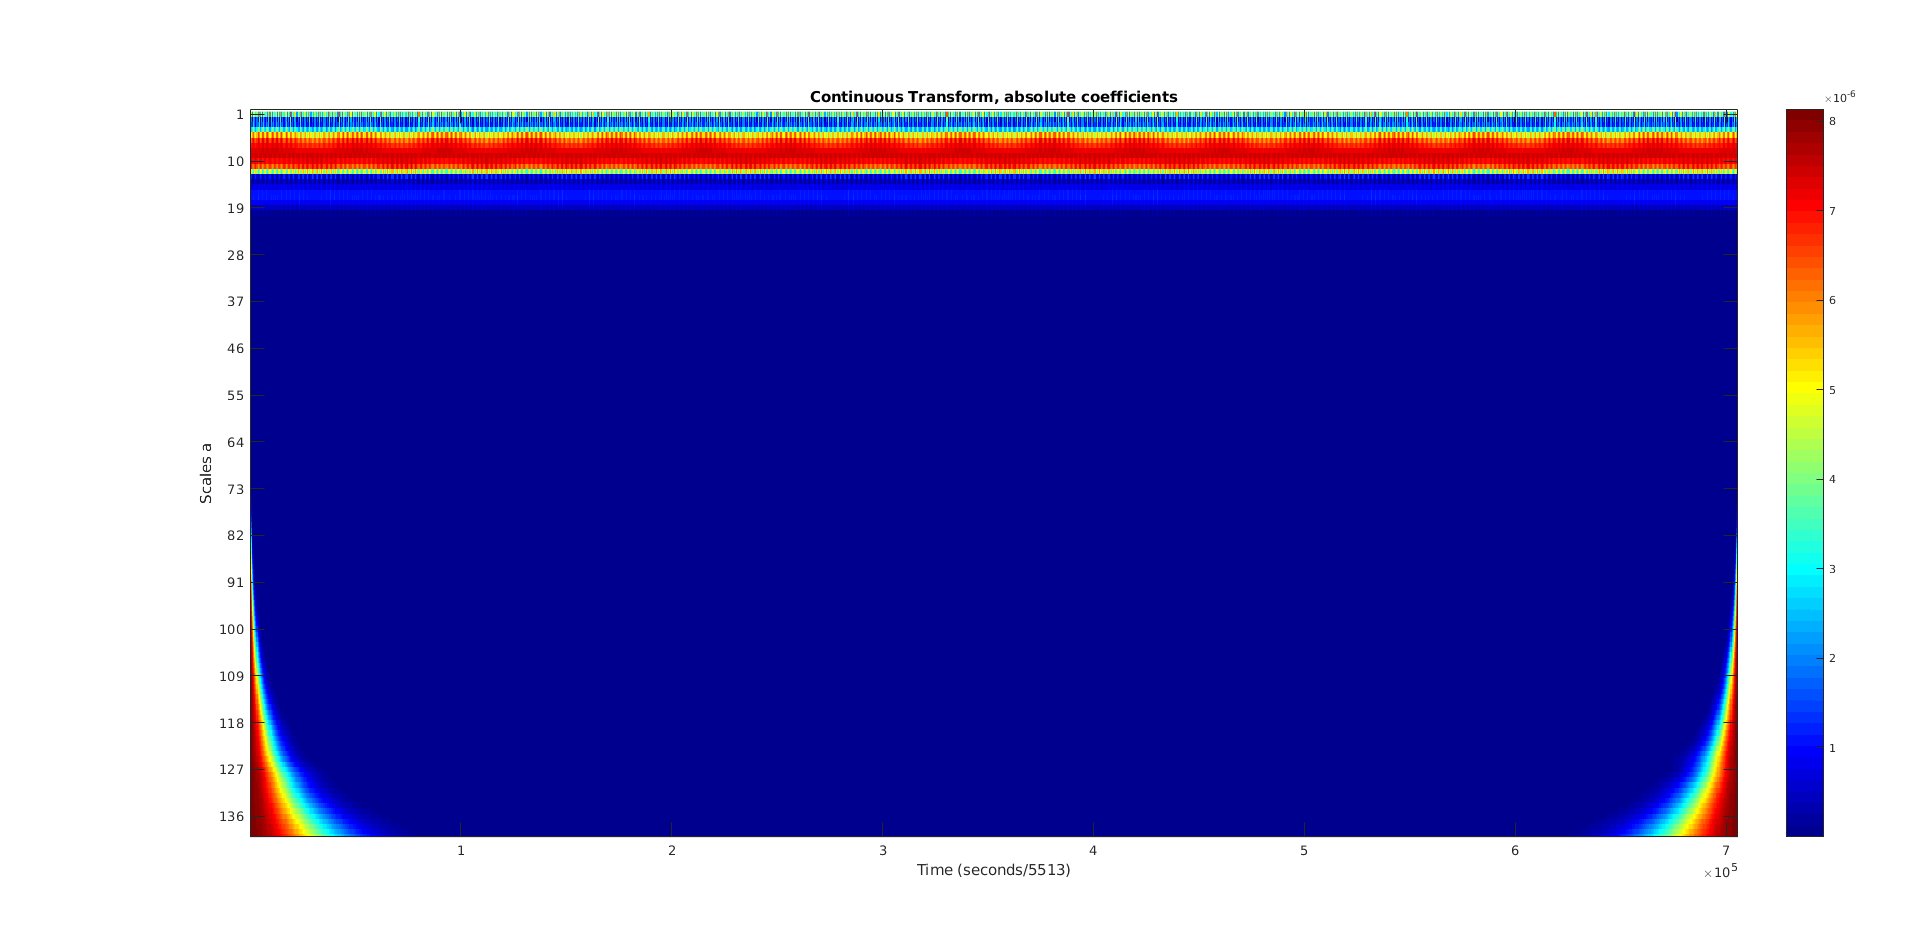
\includegraphics[width=0.9\linewidth]{papers/meteor/images/anomalie/beam/cwt_1200hz.png}
	\caption{1200 Herz Sinussignal mit kontinuierliche Wavelet-Transformation}
	\label{fig:cwt_anomalie_beam_2}
\end{figure}
Aus den durchgeführten Experimenten lässt sich erkennen, wie das am besten korrelierende Wavelet, mit zunehmender Frequenz gestaucht wird. 
Signale mit Frequenzen über 1000 Hz korrelieren mit dem Gabor-Wavelet in Skalen unter 15.
Dieser Bereich wurde bei der Radarsignalanalyse gar nicht betrachtet, da in diesem Bereich keine Auffälligkeiten sichtbar waren. 

\newpage
Um das Verhalten der Signale der Flugobjekte nachzuvollziehen, werden Signale mit ansteigenden Frequenzen von 100 Hz bis 2400 Hz untersucht:
\begin{figure}[h]
	\centering
	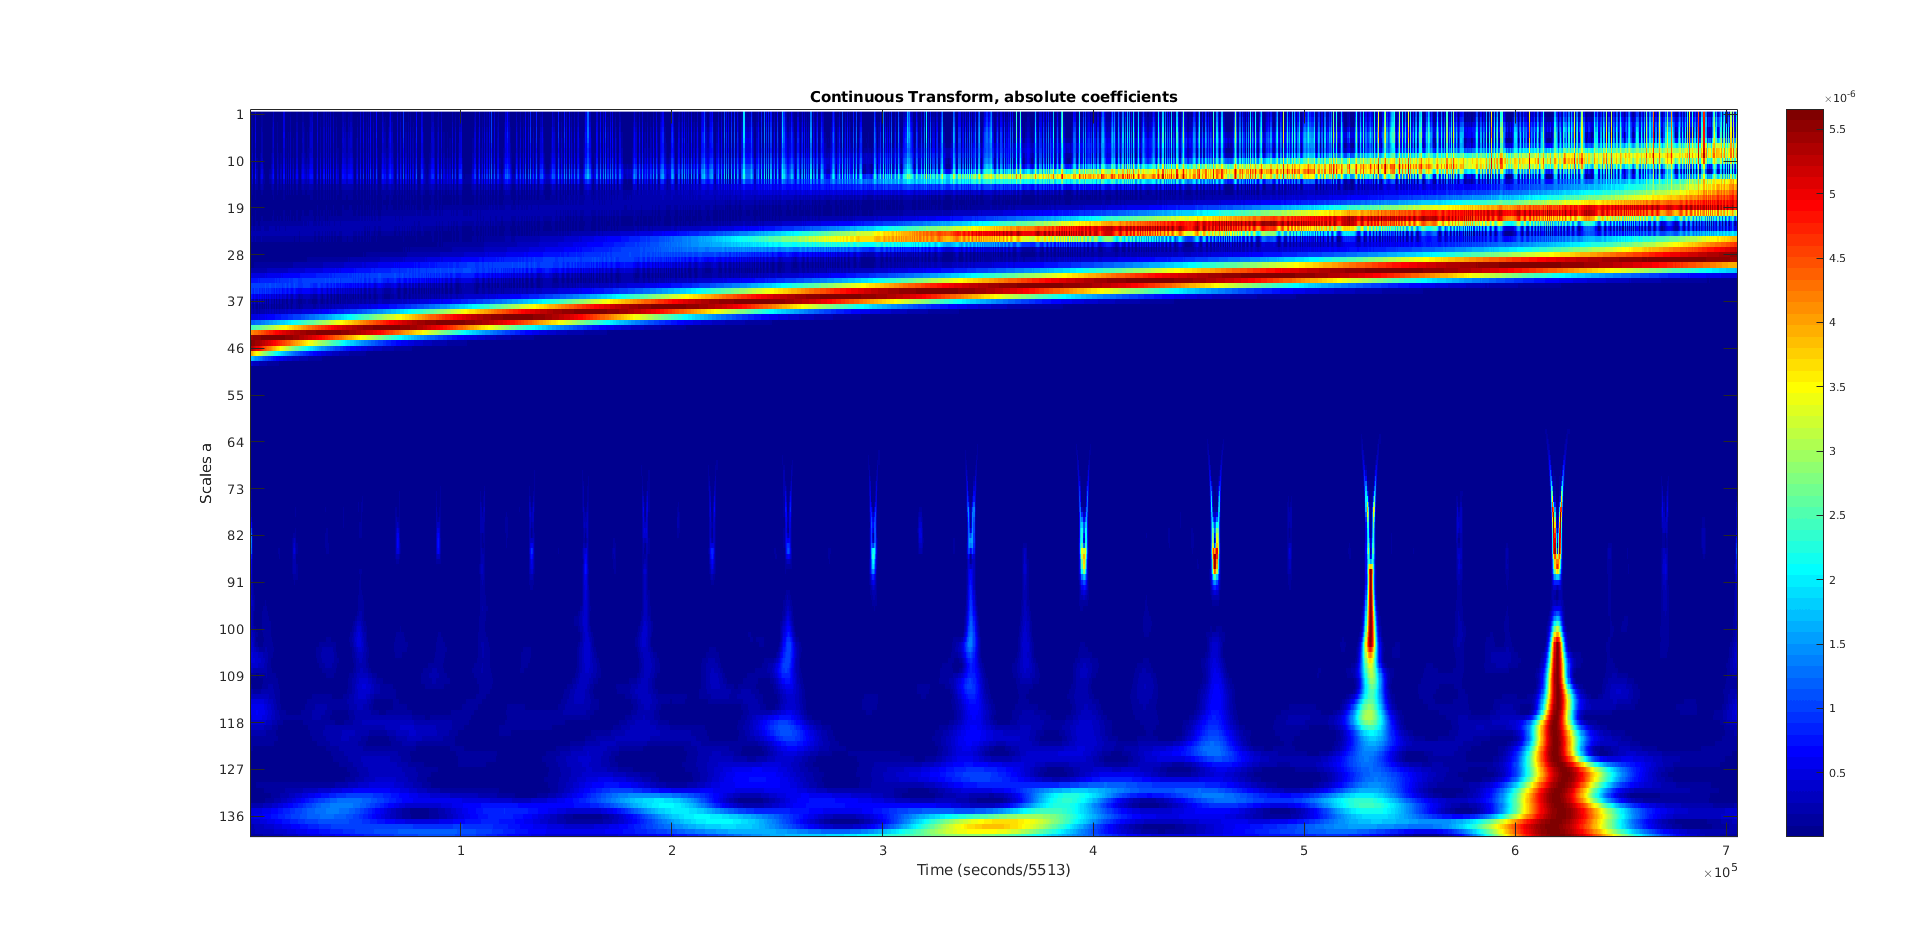
\includegraphics[width=0.9\linewidth]{papers/meteor/images/anomalie/sweep/cwt_0100to0300hz.png}
	\caption{100 bis 300 Herz Sinussignal mit kontinuierliche Wavelet-Transformation}
	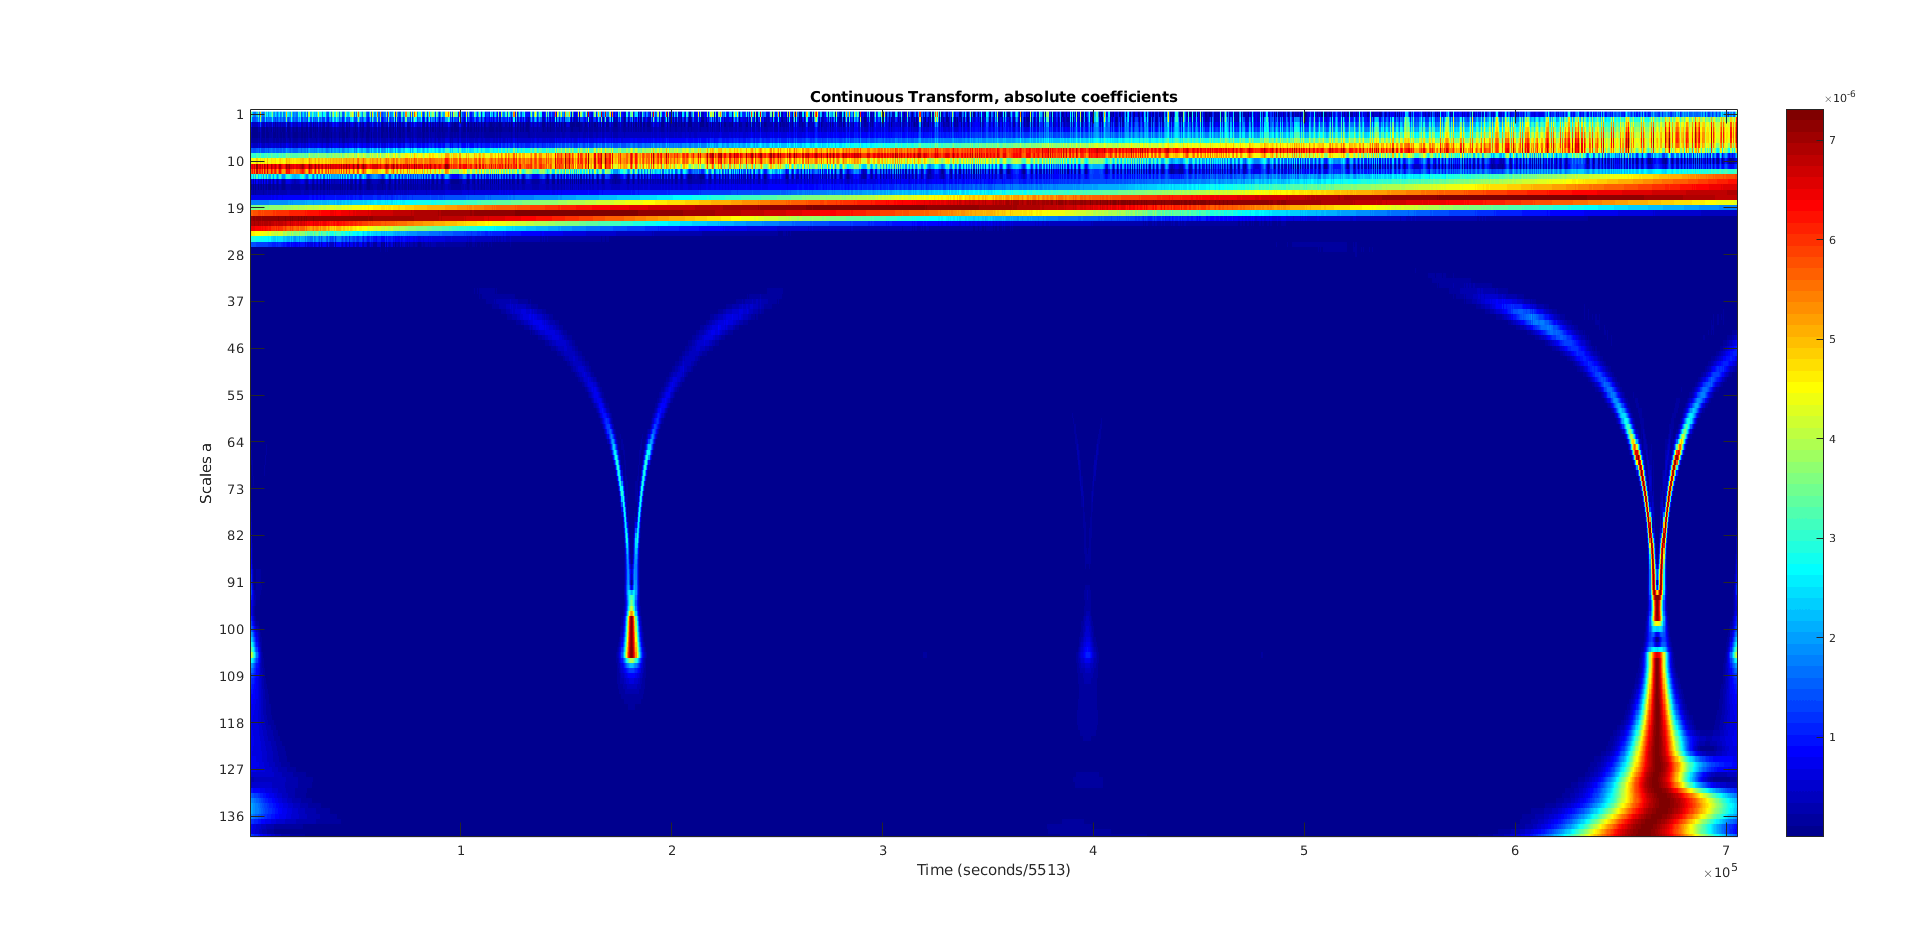
\includegraphics[width=0.9\linewidth]{papers/meteor/images/anomalie/sweep/cwt_0500to0700hz.png}
	\caption{500 bis 700 Herz Sinussignal mit kontinuierliche Wavelet-Transformation}
	\label{fig:cwt_anomalie_beam_1}
\end{figure}
\newpage
\begin{figure}[h]
	\centering
	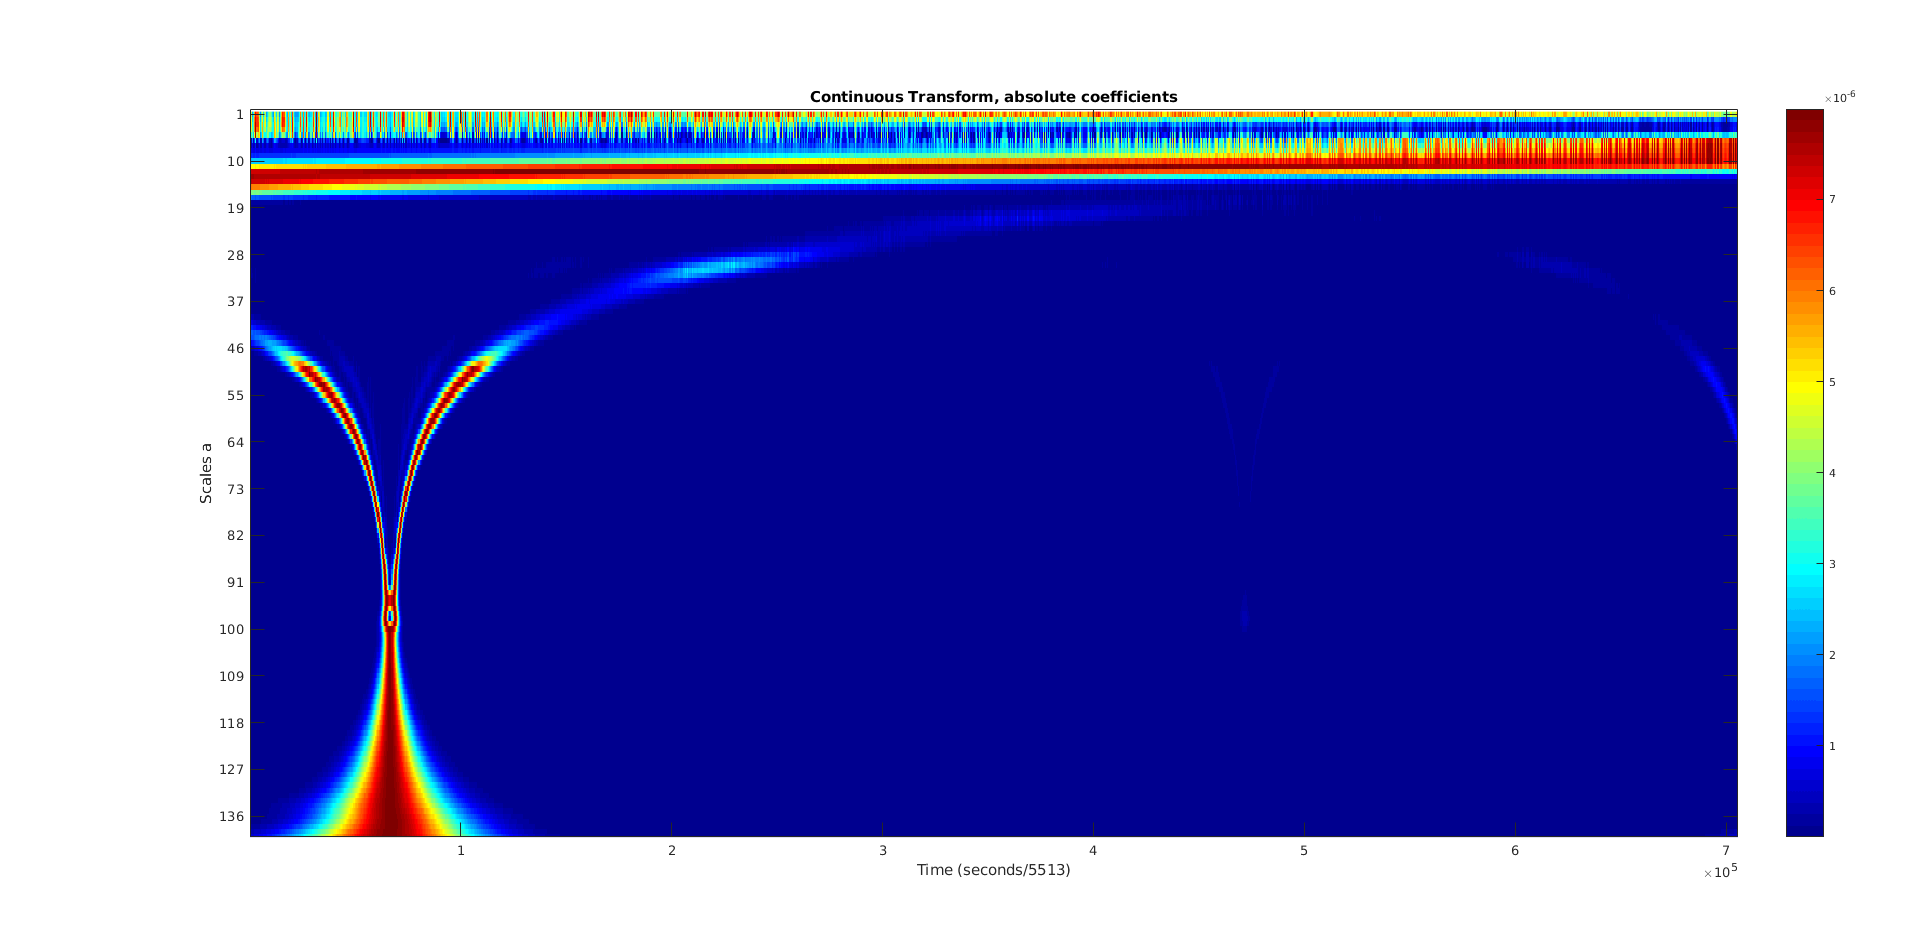
\includegraphics[width=0.9\linewidth]{papers/meteor/images/anomalie/sweep/cwt_0900to1100hz.png}
	\caption{900 bis 1100 Herz Sinussignal mit kontinuierliche Wavelet-Transformation}
	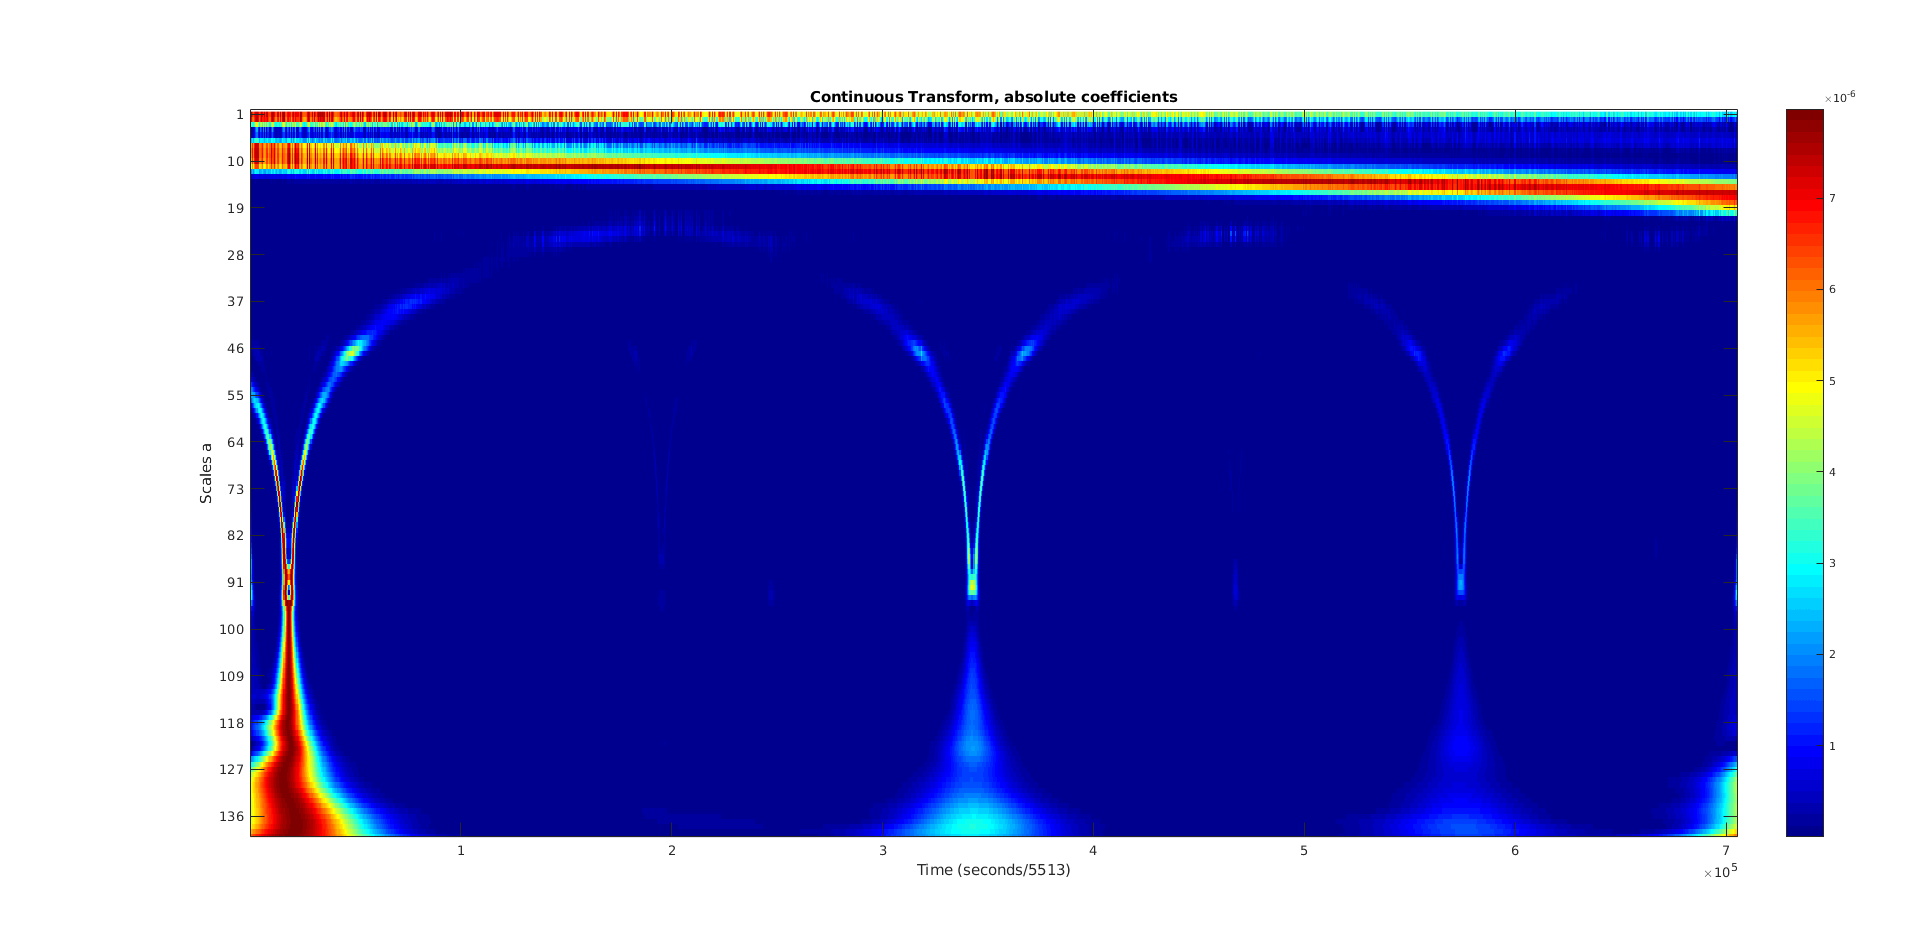
\includegraphics[width=0.9\linewidth]{papers/meteor/images/anomalie/sweep/cwt_2200to2400hz.png}
	\caption{2200 bis 2400 Herz Sinussignal mit kontinuierliche Wavelet-Transformation}
	\label{fig:cwt_anomalie_beam_2}
\end{figure}
Aus den durchgeführten Experimenten lässt sich erkennen, wie die V-förmigen Signaturen bereits bei tiefen `Sweep'-Signalen auftreten.
Anhand von 24 untersuchten `Sweep'-Signalen komme ich zum Schluss, dass die Signaturen nicht von der Frequenz abhängig sind.
Ausserdem resultieren sie nicht aus dem originalen Signal, darauf kann auch anhand der vorhergegangenen Experimente geschlossen werden, sondern einem Vielfachen der Frequenz daraus. 
Die gezogenen Schlüsse aus den Signaturen beziehen sich also nicht auf das tatsächliche Signal.

\newpage
\section{Schlussfolgerung}
\rhead{Schlussfolgerung}

Die Methode der kontinuierlichen Wavelet-Transformation und die daraus resultierende Analyse zeigt, dass diese für die Detektierung von Meteoren geeignet ist.
Anhand der entstehenden Grafiken können Meteore von anderen Flugobjekten unterschieden werden.
Den Ereignissen können sehr exakt eine Zeit zugeordnet werden.
Im Vergleich zur gefensterten Fourier-Transformation müssen weniger Parameter evaluiert werden.
Am Ende der Arbeit wurde mir bewusst, dass sich die mir charakteristisch zeigenden Signaturen nicht direkt Wavelet Korrelationen mit dem Grund-Radarsignal sind, sondern Korrelationen mit Vielfachen oder anderen Ähnlichkeiten mit der Form des Radarsignales.
Der Bereich, in dem das Gabor-Wavelet tatsächlich mit dem Radarsignal korreliert, bei circa 1000 Hz, befindet sich in der resultierenden Grafik im Bereich der Skala zwischen etwa 5 und 15.
Leider ist bei der Analyse des Radarsignals in diesem Bereich nichts sichtbar.
Meine Wavelet-Transformation ist in der derzeitigen Form nicht fähig diesen Bereich hoch genug aufzulösen, damit ein brauchbares Bild entsteht.
\begin{figure}[h!]
	\centering
	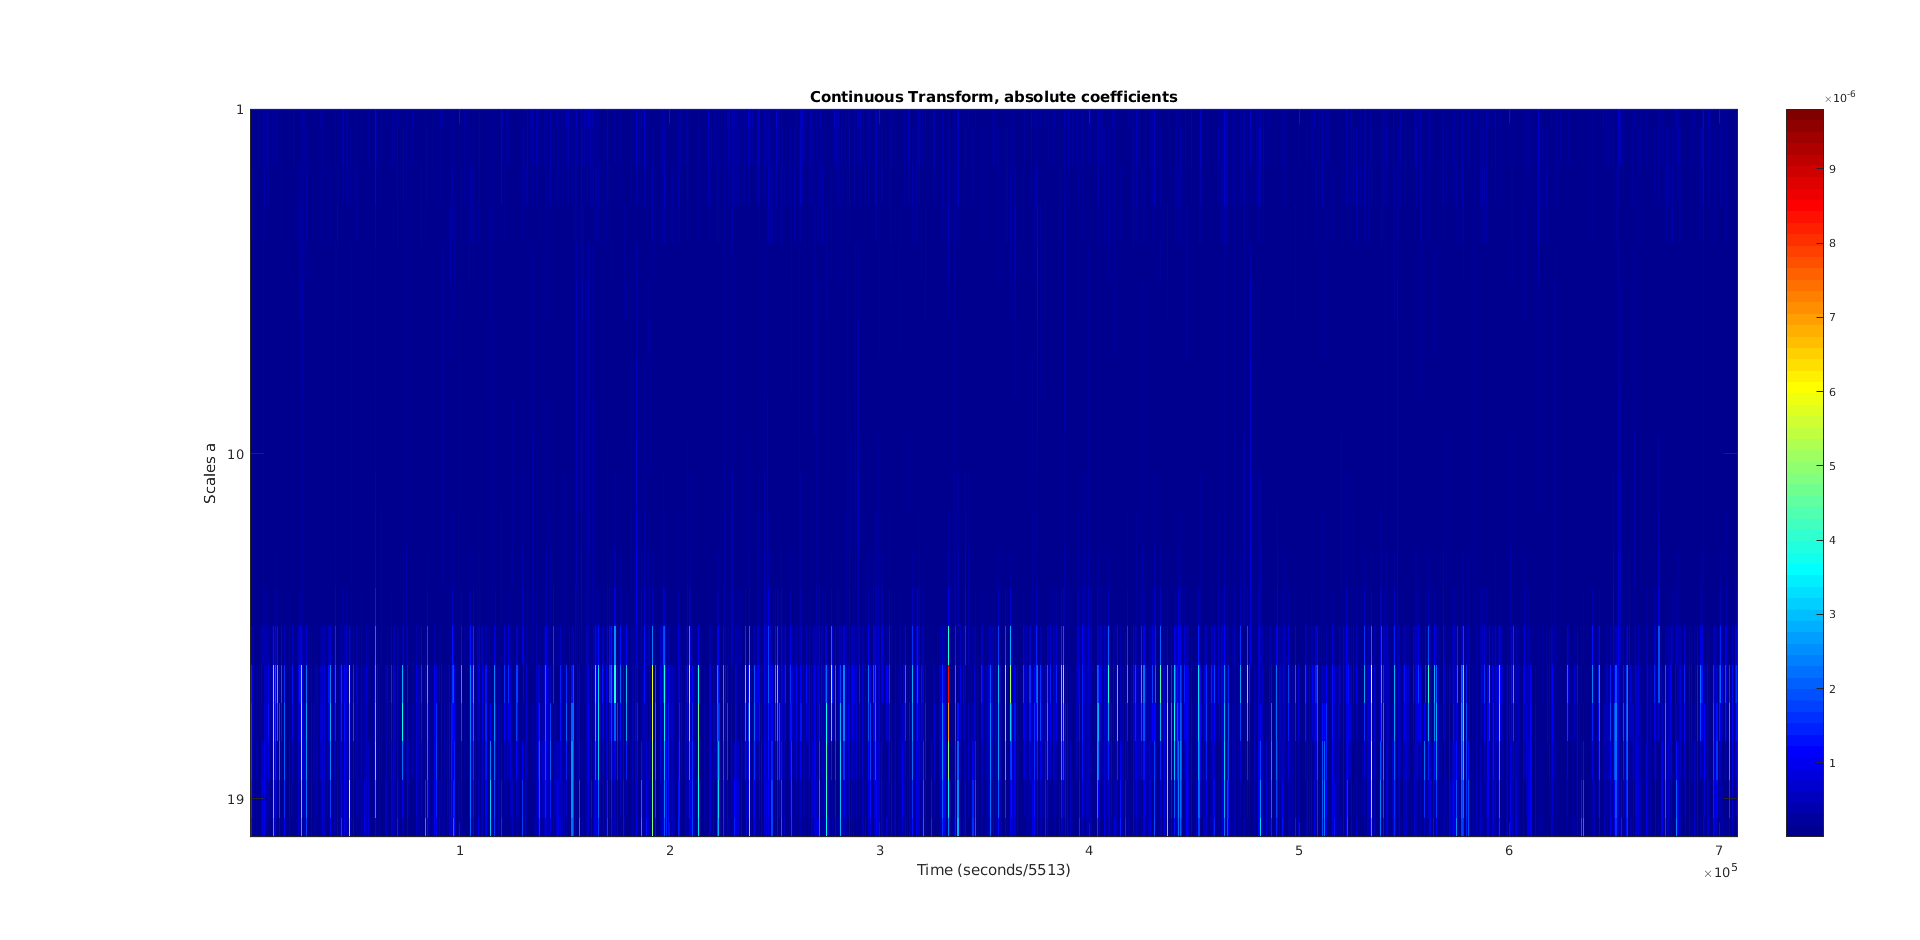
\includegraphics[width=\linewidth]{papers/meteor/images/anomalie/cwt_signal_scale1to20.png}
	\caption{Das Radarsignal aufgelöst im Bereich der Skala von 1 bis 20}
	\label{fig:signalmitwscaloscale1to20}
\end{figure}

Die kontinuierliche Wavelet-Transformation ist ausserdem sehr Rechenintensiv. 
Mit dem Programm Matlab müssen die Berechnungen sehr vorsichtig vorgenommen werden, da ansonsten der Rechner gerne zur Überlastung neigt.
Ausserdem spielt es eine grosse Rolle welche Matlab Funktionen bei der Wavelet-Transformation eingesetzt werden.
Die in diesem Abschnitt genutzten Matlab Funktionen haben sich als sehr geeignet erwiesen.  

Es grüsst Dominic Hüppi

\printbibliography[heading=subbibliography]
\end{refsection}
